\ifdefined\beamerclass
\else
    \def\beamerclass{beamer}
\fi
\documentclass[\beamerclass]{beamer}

\usepackage{pgfpages}
\mode<handout>{
	% \setbeamercolor{background canvas}{bg=black!20}
	\pgfpagesuselayout{2 on 1}[a4paper,border shrink=5mm]
}

\usepackage{lmodern}
\usepackage{listings}
\usepackage{amsmath}
\usepackage{bm}
\usepackage{textpos} % package for the positioning

\usepackage{pgf, tikz}
\usepackage{pgfplots}
\usetikzlibrary{arrows, automata}

\usetheme{Copenhagen}
\hypersetup{pdfstartview={Fit}}
\lstset{basicstyle=\small\ttfamily,breaklines=true}

\title[Differentiation]{The power of differentiation}
\author{Jonathon Hare}
\institute[]
{
  Vision, Learning and Control\\
  University of Southampton 
}
\date{}
\subject{Computer Science}
\useoutertheme{infolines}
\setbeamertemplate{headline}{} %remove headline
\setbeamertemplate{navigation symbols}{} %remove navigation symbols

\definecolor{darkblue}{RGB}{37,55,97}
\definecolor{mellowyellow}{RGB}{247,206,70}
\definecolor{almostwhite}{RGB}{254,255,255}
\definecolor{merrygreen}{RGB}{79,173,91}
\definecolor{funkyorange}{RGB}{240,154,56}

\addtobeamertemplate{footnote}{\hskip -2em}{}
\newcommand\blfootnote[1]{%
  \begingroup
  \renewcommand\thefootnote{}\footnote{#1}%
  \addtocounter{footnote}{-1}%
  \endgroup
}

\DeclareMathOperator{\softmax}{softmax}

\pgfplotsset{compat=1.17}

\begin{document}

\begin{frame}[plain]
        \begin{tikzpicture}[overlay, remember picture, shift={(current page.south west)},font={\fontfamily{Montserrat-TOsF}\selectfont}]
        \fill [funkyorange,text=darkblue] (0,0) rectangle (\paperwidth, \paperheight);
        \draw (4,7) node [align=left,text=almostwhite] {\Huge \begin{tabular}{l} \textbf{Follow} \\ \textbf{the} \\ \textbf{Gradient} \end{tabular}};
        \draw (11,1) node [align=left,text=almostwhite] {\includegraphics[scale=0.15]{../vlc.png}};
        \end{tikzpicture}
\end{frame}

\frame{
  \titlepage
}

\begin{frame}
\frametitle{Topics}
\begin{itemize}
	\item The big idea: optimisation by following gradients
	\item Recap: what are gradients and how do we find them?
	\item Recap: Singular Value Decomposition and its applications
	\item Example: Computing SVD using gradients - The Netflix Challenge
\end{itemize}
\end{frame}

\begin{frame}
\frametitle{The big idea: optimisation by following gradients}
\begin{itemize}
	\item<+-> Fundamentally, we're interested in machines that we train by optimising parameters
	\begin{itemize}
		\item<+-> How do we select those parameters?
	\end{itemize}
	\item<+-> In deep learning/differentiable programming we typically define an objective function that we \emph{minimise} (or \emph{maximise}) with respect to those parameters
	\item<+-> This implies that we're looking for points at which the gradient of the objective function is zero w.r.t the parameters
\end{itemize}
\end{frame}

\begin{frame}
\frametitle{The big idea: optimisation by following gradients}
\begin{itemize}
	\item<+-> Gradient based optimisation is a \emph{big} field!
	\begin{itemize}
		\item<+-> First order methods, second order methods, subgradient methods...
	\end{itemize}
	\item<+-> With deep learning we're primarily interested in first-order methods\only<3->{\footnote{Second order gradient optimisers are potentially better, but for systems with many variables are currently impractical as they require computing the Hessian.}}.
	\begin{itemize}
		\item<+-> Primarily using variants of gradient descent: a function $F(\bm x)$ has \emph{a} minima\only<4->{\footnote{not necessarily global or unique}} (or a saddle-point) at a point $\bm x = \bm a$ where $\bm a$ is given by applying $\bm{a}_{n+1} = \bm a_n - \alpha \nabla F(\bm a_n)$ until convergence from some initial point $\bm a_0$.
	\end{itemize}
\end{itemize}
\end{frame}

% \begin{frame}
% \frametitle{The big idea: optimisation by following gradients}
% \framesubtitle{A simple 1D example}
% \end{frame}

% \begin{frame}
% \frametitle{The big idea: optimisation by following gradients}
% \framesubtitle{A simple 2D example}
% \end{frame}

% \begin{frame}
% \frametitle{The big idea: optimisation by following gradients}
% \framesubtitle{A more indicative example}
% \end{frame}

\begin{frame}
\frametitle{Recap: what are gradients and how do we find them?}
\framesubtitle{The derivative in 1D}
\begin{columns}
\begin{column}{0.65\textwidth}
\begin{itemize}
	\item<+-> Recall that the gradient of a straight line is $\frac{\Delta y}{\Delta x}$.
	\item<+-> For an arbitrary real-valued function, $f(a)$, we can approximate the derivative, $f'(a)$ using the gradient of the \emph{secant line} defined by $(a,f(a))$ and a point a small distance, $h$, away $(a+h,f(a+h))$: $f'(a) \approx \frac{f(a+h) - f(a)}{h}$.
	\begin{itemize}
		\item<+-> This expression is `Newton's Quotient' or `Fermat's Difference Quotient'.
		\item<+-> As $h$ becomes smaller, the approximated derivative becomes more accurate. 
		\item<+-> If we take the limit as $h \to 0$, then we have an exact expression for the derivative: $\frac{df}{da} = f'(a) = \lim_{h\to0} \frac{f(a+h) - f(a)}{h}$.
	\end{itemize}
\end{itemize}
\end{column}
\begin{column}{0.35\textwidth}

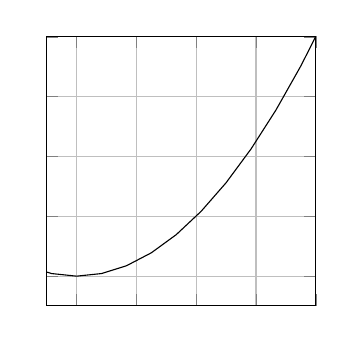
\begin{tikzpicture}
	\begin{axis}[
		height=5cm,
		width=5cm,
		grid=both,
		xtick distance=1,
		ytick distance=1,
		xticklabels={,,},
		yticklabels={,,},
		axis equal,
		xmin=-0.5,
		xmax=4 
	]
		
	\addplot[]{0.25*x^2};
	\end{axis}
\end{tikzpicture}

\end{column}
\end{columns}
\end{frame}

\begin{frame}
\frametitle{Recap: what are gradients and how do we find them?}
\framesubtitle{The derivative of $y=x^2$ from first principles}
\begin{align*}
    \onslide<+->{y &= x^2 \\}
    \onslide<+->{\frac{dy}{dx} &= \lim_{h\to0} \frac{(x+h)^2 - x^2}{h} \\}
    \onslide<+->{\frac{dy}{dx} &= \lim_{h\to0} \frac{x^2 + h^2 + 2hx - x^2}{h} \\}
    \onslide<+->{\frac{dy}{dx} &= \lim_{h\to0} \frac{h^2 + 2hx}{h} \\}
    \onslide<+->{\frac{dy}{dx} &= \lim_{h\to0} (h + 2x) \\}
    \onslide<+->{\frac{dy}{dx} &= 2x}
\end{align*}
\end{frame}

\begin{frame}
\frametitle{Recap: what are gradients and how do we find them?}
\framesubtitle{Aside: numerical approximation of the derivative}

\begin{columns}
\begin{column}{0.65\textwidth}
% central difference as opposed to one sided
\begin{itemize}
\item For numerical computation of derivatives it is better to use a ``centralised'' definition of the derivative:
\begin{itemize}
	\item<+-> $f'(a) = \lim_{h\to0} \frac{f(a+h) - f(a-h)}{2h}$
	\item<+-> The bit inside the limit is known as the \emph{symmetric difference quotient}
	\item<+-> For small values of $h$ this has less error than the standard one-sided difference quotient.
\end{itemize}
\end{itemize}

\end{column}
\begin{column}{0.35\textwidth}

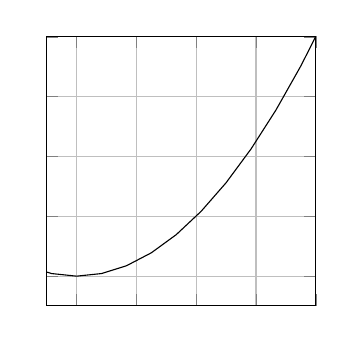
\begin{tikzpicture}
	\begin{axis}[
		height=5cm,
		width=5cm,
		grid=both,
		xtick distance=1,
		ytick distance=1,
		xticklabels={,,},
		yticklabels={,,},
		axis equal,
		xmin=-0.5,
		xmax=4 
	]
		
	\addplot[]{0.25*x^2};
	\end{axis}
\end{tikzpicture}

\end{column}
\end{columns}
\end{frame}


\begin{frame}
\frametitle{Recap: what are gradients and how do we find them?}
\framesubtitle{Aside: numerical approximation of the derivative}
\begin{itemize}
\item<+-> If you are going to use difference quotients to estimate derivatives you need to be aware of potential rounding errors due to floating point representations.
\begin{itemize}
	\item Calculating derivatives this way using less than 64-bit precision is rarely going to be useful. (Numbers are not represented exactly, so even if $h$ is represented exactly, $x+h$ will probably not be)
	\item You need to pick an appropriate $h$ - too small and the subtraction will have a large rounding error!
\end{itemize}
\end{itemize}
\end{frame}

\begin{frame}
\frametitle{Recap: what are gradients and how do we find them?}
\framesubtitle{Derivatives of deeper functions}

\begin{itemize}
	\item<+-> Deep learning is all about optimising deeper functions; functions that are compositions of other functions
	\begin{itemize}
		\item e.g. $z = f \circ g(x) = f(g(x))$
	\end{itemize}
	\item<+-> The chain rule of calculus tells us how to differentiate compositions of functions:
	\begin{itemize}
		\item $\frac{dz}{dx}=\frac{dz}{dy}\frac{dy}{dx}$
	\end{itemize}
\end{itemize}
\end{frame}

\begin{frame}
\frametitle{Recap: what are gradients and how do we find them?}
\framesubtitle{Example: differentiating $z=x^4$}

{\small Note that this is a silly example that just serves to demonstrate the principle!}
\begin{align*}
    \onslide<+->{z &= x^4 \\}
    \onslide<+->{z &= (x^2)^2 = y^2 \quad{\rm where}\quad y=x^2 \\}
    \onslide<+->{\frac{dz}{dx} &= \frac{dz}{dy}\frac{dy}{dx} = (2y) (2x) = (2x^2) (2x) = 4x^3}
\end{align*}
\uncover<+->{
Equivalently, from first principles:
\begin{align*}
    z &= x^4 \\
    \frac{dz}{dx} &= \lim_{h\to0} \frac{(x+h)^4 - x^4}{h} \\
    \frac{dz}{dx} &= \lim_{h\to0} \frac{h^4 + 4 h^3 x + 6 h^2 x^2 + 4 h x^3 + x^4 - x^4}{h} \\
    % \onslide<+->{\frac{dz}{dx} &= \lim_{h\to0} \frac{h^4 + 4 h^3 x + 6 h^2 x^2 + 4 h x^3}{h} \\}
    \frac{dz}{dx} &= \lim_{h\to0} h^3 + 4 h^2 x + 6 h x^2 + 4 x^3 = 4 x^3\\
\end{align*}
}
\end{frame}

\begin{frame}
\frametitle{Recap: what are gradients and how do we find them?}
\framesubtitle{Vector functions}
\begin{itemize}
	\item<+-> What if we're dealing with a \emph{vector} function, $\bm y(t)$?
	\begin{itemize}
		\item<+-> This can be split into its constituent coordinate functions: $\bm y(t) = (y_1(t),\dots,y_n(t))$.
		\item<+-> Thus the derivative is a vector (the `tangent vector'), $\bm y'(t)=(y_1'(t),\dots,y_n'(t))$, which consists of the derivatives of the coordinate functions.
		\item<+-> Equivalently, $\bm y'(t) = \lim_{h\to0} \frac{\bm y(t+h) - \bm y(t)}{h}$ if the limit exists.
	\end{itemize}
\end{itemize}
\end{frame}

\begin{frame}
\frametitle{Recap: what are gradients and how do we find them?}
\framesubtitle{Functions of multiple variables: partial differentiation}

\begin{itemize}
	\item What if the function we're trying to deal with has multiple variables\footnote{A multivariate function} (e.g. $f(x, y) = x^2 + xy + y^2$)?
	\begin{itemize}
		\item<+-> This expression has a pair of \emph{partial derivatives}, $\frac{\partial f}{\partial x} = 2x+y$ and $\frac{\partial f}{\partial y} = x + 2y$, computed by differentiating with respect to each variable $x$ and $y$ whilst holding the other(s) constant.
	\end{itemize}
	\item<+-> In general, the partial derivative of a function $f(x_1,\dots,x_n)$ at a point $(a_1,\dots,a_n)$ is given by: \\ $\frac{\partial f}{\partial x_i}(a_1,\dots,a_n) = \lim_{h\to0}\frac{f(a_1\dots,a_i+h,\dots,a_n)-f(a_1\dots,a_i,\dots,a_n)}{h}$.
	\item<+-> The vector of partial derivatives of a scalar-value multivariate function, $f(x_1,\dots,x_n)$ at a point $(a_1,\dots,a_n)$, can be arranged into a vector:
	$\nabla f(a_1,\dots,a_n) = \big(\frac{\partial f}{\partial x_1}(a_1,\dots,a_n), \dots, \frac{\partial f}{\partial x_n}(a_1,\dots,a_n) \big)$.
	\begin{itemize}
		\item<+-> This is the \textbf{gradient} of $f$ at $a$.
	\end{itemize}
	\item<+-> In the case of a vector-valued multivariate function, the partial derivatives form a matrix called the \textbf{Jacobian}.
\end{itemize}
\end{frame}

\begin{frame}
\frametitle{Recap: what are gradients and how do we find them?}
\framesubtitle{Functions of vectors and matrices: partial differentiation}
\begin{itemize}
	\item<+-> For the kinds of functions (and programs) that we'll look at \emph{optimising} in this course have a number of typical properties:
	\begin{itemize}
		\item<+-> They are scalar-valued
		\begin{itemize}
			\item We'll look at programs with \emph{multiple losses}, but ultimately we can just consider optimising with respect to the \emph{sum} of the losses.
		\end{itemize}
		\item<+-> They involve multiple variables, which are often wrapped up in the form of vectors or matrices, and more generally tensors.
		\item<+-> \textbf{How will we find the gradients of these?}
	\end{itemize}
\end{itemize}
\end{frame}

\begin{frame}
\frametitle{Recap: what are gradients and how do we find them?}
\framesubtitle{The chain rule for vectors}
\uncover<+->{
Suppose that $\bm x \in \mathbb{R}^m$, $\bm y \in \mathbb{R}^n$, $g$ maps from $\mathbb{R}^m$ to $\mathbb{R}^n$ and $f$ maps from $\mathbb{R}^n$ to $\mathbb{R}$.
}

\uncover<+->{
If $\bm y = g(\bm x)$ and $z = f(\bm y)$, then \\
\begin{align*}
	\frac{\partial z}{\partial x_i} &= \sum_j \frac{\partial z}{\partial y_j} \frac{\partial y_j}{\partial x_i}.
\end{align*}
}

\uncover<+->{
Equivalently, in vector notation: \\
\begin{align*}
	\nabla_{\bm x}z &= (\frac{\partial \bm y}{\partial \bm x})^\top \nabla_{\bm y}z
\end{align*}
where $\frac{\partial \bm y}{\partial \bm x}$ is the $n \times m$ Jacobian matrix of $g$.
}

\end{frame}

\begin{frame}
\frametitle{Recap: what are gradients and how do we find them?}
\framesubtitle{The chain rule for Tensors}
\begin{itemize}
	\item<+-> Conceptually, the simplest way to think about gradients of tensors is to imagine flattening them into vectors, computing the vector-valued gradient and then reshaping the gradient back into a tensor. 
	\begin{itemize}
		\item<+-> In this way we're still just multiplying Jacobians by gradients. 
	\end{itemize}
	\item<+-> More formally, consider the gradient of a scalar $z$ with respect to a tensor $\mathbf{X}$ to be denoted as $\nabla_{\mathbf{X}}z$. 
	\begin{itemize}
		\item<+-> Indices into $\mathbf{X}$ now have multiple coordinates, but we can generalise by using a single variable $i$ to represent the complete tuple of indices. 
		\begin{itemize}
			\item<+-> For all index tuples $i$, $(\nabla_{\mathbf{X}}z)_i$ gives $\frac{\partial z}{\partial \mathsf{X}_i}$.
		\end{itemize}
		\item<+-> Thus, if $\mathbf{Y} = g(\mathbf{X})$ and $z = f(\mathbf{Y})$ then $\nabla_{\mathbf{X}}z = \sum_j (\nabla_{\mathbf{X}}\mathsf{Y}_j)\frac{\partial z}{\partial \mathsf{Y}_j}$.
	\end{itemize}
\end{itemize}


\end{frame}

\begin{frame}
\frametitle{Recap: what are gradients and how do we find them?}
\framesubtitle{Example: $\nabla_{\bm W} f(\bm X \bm W)$}
\begin{itemize}
\item<1-> Let $\bm D = \bm X \bm W$ where the rows of $\bm X \in \mathbb{R}^{n \times m}$ contain some fixed \emph{features}, and $\bm W \in \mathbb{R}^{m \times h}$ is a matrix of weights.
\item<1-> Also let $\mathcal{L} = f(\bm D)$ be some scalar function of $\bm D$ that we wish to minimise. 
\item<2-> What are the derivatives of $\mathcal{L}$ with respect to the weights $\bm W$?
\end{itemize}
\end{frame}

\begin{frame}
\frametitle{Recap: what are gradients and how do we find them?}
\framesubtitle{Example: $\nabla_{\bm W} f(\bm X \bm W)$}
\begin{itemize}
	\item<+-> Start by considering a specific weight, $W_{uv}$: 
$\frac{\partial \mathcal{L}}{\partial W_{uv}} = \sum_{i,j}\frac{\partial \mathcal{L}}{\partial D_{ij}}\frac{\partial D_{ij}}{\partial W_{uv}}$.
	\item<+-> We know that $\frac{\partial D_{ij}}{\partial W_{uv}}=0$ if $j \neq v$ because $D_{ij}$ is the dot product of row $i$ of $\bm X$ and column $j$
 of $\bm W$.
 	\item<+-> Therefore, we can simplify the summation to only consider cases where $j=v$: $\sum_{i,j}\frac{\partial \mathcal{L}}{\partial D_{ij}}\frac{\partial D_{ij}}{\partial W_{uv}} = \sum_i \frac{\partial \mathcal{L}}{\partial D_{iv}}\frac{\partial D_{iv}}{\partial W_{uv}}$.
 	\item<+-> What is $\frac{\partial D_{iv}}{\partial W_{uv}}$?
 		\begin{align*}
 			\uncover<+->{D_{iv} &= \sum_{k=1}^{m} X_{ik} W_{kv} \\}
 			\uncover<+->{\frac{\partial D_{iv}}{\partial W_{uv}} &= \frac{\partial}{\partial W_{uv}} \sum_{k=1}^{m} X_{ik} W_{kv} = \sum_{k=1}^{m} \frac{\partial}{\partial W_{uv}} X_{ik} W_{kv} \\}
 			\uncover<+->{\therefore \frac{\partial D_{iv}}{\partial W_{uv}} &= X_{iu} \\}
 		\end{align*}
\end{itemize}
\end{frame}

\begin{frame}
\frametitle{Recap: what are gradients and how do we find them?}
\framesubtitle{Example: $\nabla_{\bm W} f(\bm X \bm W)$}
\begin{itemize}
	\item<+-> Putting every together, we have: $\frac{\partial \mathcal{L}}{\partial W_{uv}} = \sum_{i}\frac{\partial \mathcal{L}}{\partial D_{iv}}X_{iu}$.
	\item<+-> As we're summing over multiplications of scalars, we can change the order: $\frac{\partial \mathcal{L}}{\partial W_{uv}} = \sum_{i}X_{iu}\frac{\partial \mathcal{L}}{\partial D_{iv}}$.
	\item<+-> and note that the sum over $i$ is doing a dot product with row $u$ and column $v$ if we transpose $X_{iu}$ to $X^\top_{ui}$: $\frac{\partial \mathcal{L}}{\partial W_{uv}} = \sum_{i}X^\top_{ui}\frac{\partial \mathcal{L}}{\partial D_{iv}}$.
	\item<+-> \vspace{5mm} We can then see that if we want this for all values of $\bm W$ it simply generalises to: $\frac{\partial \mathcal{L}}{\partial \bm W} = \bm X^\top\frac{\partial \mathcal{L}}{\partial \bm D}$.
\end{itemize}
\end{frame}


\begin{frame}
\frametitle{Recap: what are gradients and how do we find them?}
\framesubtitle{STOP! What does a gradient actually mean?}

\begin{itemize}
	\item<+-> In your early calculus lessons you likely had it hammered into you that gradients represent rates of change of functions.
	\item<+-> This is of course totally true...
	\item<+-> But, it isn't a particularly useful way to think about the gradients of a loss with respect to the weights of a parameterised function.
	\begin{itemize}
		\item<+-> \textbf{The gradient of the loss with respect to a parameter tells you how much the loss will change with a small perturbation to that parameter.}
	\end{itemize}
\end{itemize}

\end{frame}

\begin{frame}
\frametitle{Recap: Singular Value Decomposition and its applications}
Let's now change direction --- we're going to look at an early success story resulting from using some differentiation and the Singular Value Decomposition (SVD).
\\[1em]
For complex $\bm A:$ \\
\begin{align*}
\bm A &= \bm U \bm \Sigma \bm V^*
\end{align*}
where $\bm V^*$ is the \emph{conjugate transpose} of $\bm V$.\\[1em]
For real $\bm A:$ \\
\begin{align*}
\bm A &= \bm U \bm \Sigma \bm V^\top
\end{align*}
\end{frame}

\begin{frame}
\frametitle{Recap: Singular Value Decomposition and its applications}
\begin{itemize}
	\item SVD has many uses:
	\begin{itemize}
		\uncover<+->{
		\item Computing the Eigendecomposition:
		\begin{itemize}
			\item Eigenvectors of $\bm A\bm A^\top$ are columns of $\bm U$,
			\item Eigenvectors of $\bm A^\top\bm A$ are columns of $\bm V$,
			\item and the non-zero values of $\bm\Sigma$ are the square roots of the non-zero eigenvalues of both $\bm A\bm A^\top$ and $\bm A^\top\bm A$.
		\end{itemize}}
		\uncover<+->{
		\item Dimensionality reduction
		\begin{itemize}
			\item ...use to compute PCA
		\end{itemize}}
		\uncover<+->{
		\item Computing the Moore-Penrose Pseudoinverse
		\begin{itemize}
			\item for real $\bm A$: $\bm A^+ = \bm V \bm\Sigma^+ \bm U^\top$ where $\bm\Sigma^+$ is formed by taking the reciprocal of every non-zero diagonal element and transposing the result.
		\end{itemize}}
		\uncover<+->{
		\item<+-> Low-rank approximation and matrix completion
		\begin{itemize}
			\item if you take the $\rho$ columns of $\bm U$, and the $\rho$ rows of $\bm V^\top$ corresponding to the $\rho$ largest singular values, you can form the matrix $\bm A_\rho = \bm U_\rho \bm \Sigma_\rho \bm V^\top_\rho$ which will be the $best$ rank-$\rho$ approximation of the original $\bm A$ in terms of the Frobenius norm.
		\end{itemize}}
	\end{itemize}
\end{itemize}
\end{frame}

\begin{frame}
\frametitle{Example: Computing SVD using gradients - The Netflix Challenge}
\begin{itemize}
	\uncover<+->{\item There are many standard ways of computing the SVD:
	\begin{itemize}
		\item e.g. `Power iteration', or `Arnoldi iteration' or `Lanczos algorithm' coupled with the `Gram-Schmidt process' for orthonormalisation
	\end{itemize}}
	\uncover<+->{\item but, these don't necessarily scale up to really big problems
	\begin{itemize}
		\item e.g. computing the SVD of a sparse matrix with 17770 rows, 480189 columns and 100480507 non-zero entries!
		\item this corresponds to the data provided by Netflix when they launched the \emph{Netflix Challenge} in 2006. 
	\end{itemize}}
	\item<+-> OK, so what can you do?
	\begin{itemize}
		\item<+-> The `Simon Funk' solution: realise that there is a really simple (and quick) way to compute the SVD by following gradients...
	\end{itemize}
\end{itemize}
\end{frame}

\begin{frame}
\frametitle{Example: Computing SVD using gradients - The Netflix Challenge}
\framesubtitle{Deriving a gradient-descent solution to SVD}
\begin{itemize}
	\item<+-> One of the definitions of rank-$\rho$ SVD of a matrix $\bm A$ is that it minimises reconstruction error in terms of the Frobenius norm.
	\item<+-> Without loss of generality we can write SVD as a 2-matrix decomposition $\bm A = \hat{\bm U} \hat{\bm V}^T$ by rolling in the square roots of $\bm\Sigma$ to both $\hat{\bm U}$ and $\hat{\bm V}$: $\hat{\bm U} = \bm U \bm\Sigma^{0.5}$ and $\hat{\bm V}^\top = \bm \Sigma^{0.5} \bm V^\top$.
	\item<+-> Then we can define the decomposition as finding $\min\limits_{\hat{\bm U}, \hat{\bm V}}( \| \bm A - \hat{\bm U}\hat{\bm V}^\top \|_{\rm F}^2 )$
\end{itemize}
\end{frame}


\begin{frame}
\frametitle{Example: Computing SVD using gradients - The Netflix Challenge}
\framesubtitle{Deriving a gradient-descent solution to SVD}
\uncover<+->{
Start by expanding our optimisation problem:

\begin{align*}
	\min\limits_{\hat{\bm U}, \hat{\bm V}}( \| \bm A - \hat{\bm U}\hat{\bm V}^\top \|_{\rm F}^2 ) &= \min\limits_{\hat{\bm U}, \hat{\bm V}}( \sum_r \sum_c (A_{rc} - \hat{U}_r\hat{V}_c)^2 )	\\
			  &= \min\limits_{\hat{\bm U}, \hat{\bm V}}( \sum_r \sum_c (A_{rc} - \sum_{p=1}^{\rho}\hat{U}_{rp}\hat{V}_{cp})^2 )	 
\end{align*}
}

\uncover<+->{Let $e_{rc} = A_{rc} - \sum_{p=0}^{\rho}\hat{U}_{rp}\hat{V}_{cp}$ denote the error. Then, our problem becomes:

\begin{align*}
{\rm Minimise}\,J &= \sum_r \sum_c e_{rc}^2
\end{align*}

We can then differentiate with respect to specific variables $\hat{U}_{rq}$ and $\hat{V}_{cq}$
}
\end{frame}


\begin{frame}
\frametitle{Example: Computing SVD using gradients - The Netflix Challenge}
\framesubtitle{Deriving a gradient-descent solution to SVD}
\uncover<+->{
We can then differentiate with respect to specific variables $\hat{U}_{rq}$ and $\hat{V}_{cq}$:
\begin{align*}
	\frac{\partial J}{\partial \hat{U}_{rq}} &= \sum_r \sum_c 2e_{rc} \frac{\partial e}{\partial \hat{U}_{rq}} = -2 \sum_r \sum_c \hat{V}_{cq}e \\
	\frac{\partial J}{\partial \hat{V}_{cq}} &= \sum_r \sum_c 2e_{rc} \frac{\partial e}{\partial \hat{V}_{cq}} = -2 \sum_r \sum_c \hat{U}_{rq}e \\
\end{align*}
}

\uncover<+->{
and use this as the basis for a gradient descent algorithm:

\begin{align*}
	\hat{U}_{rq} &\Leftarrow \hat{U}_{rq} + \lambda \sum_r \sum_c \hat{V}_{cq}e_{rc} \\
	\hat{V}_{cq} &\Leftarrow \hat{V}_{cq} + \lambda \sum_r \sum_c \hat{U}_{rq}e_{rc}
\end{align*}
}

\end{frame}

\begin{frame}
\frametitle{Example: Computing SVD using gradients - The Netflix Challenge}
\framesubtitle{Deriving a gradient-descent solution to SVD}

\begin{itemize}
	\item<+-> A stochastic version of this algorithm (updates on one single item of $\bm A$ at a time) helped win the Netflix Challenge competition in 2009.
	\item<+-> It was both \emph{fast} and \emph{memory efficient}
\end{itemize}

\end{frame}

\end{document}